\subsection{Baza XML}



\subsubsection{Schemat dokumentu}
\begin{figure}[h]
 \centering
 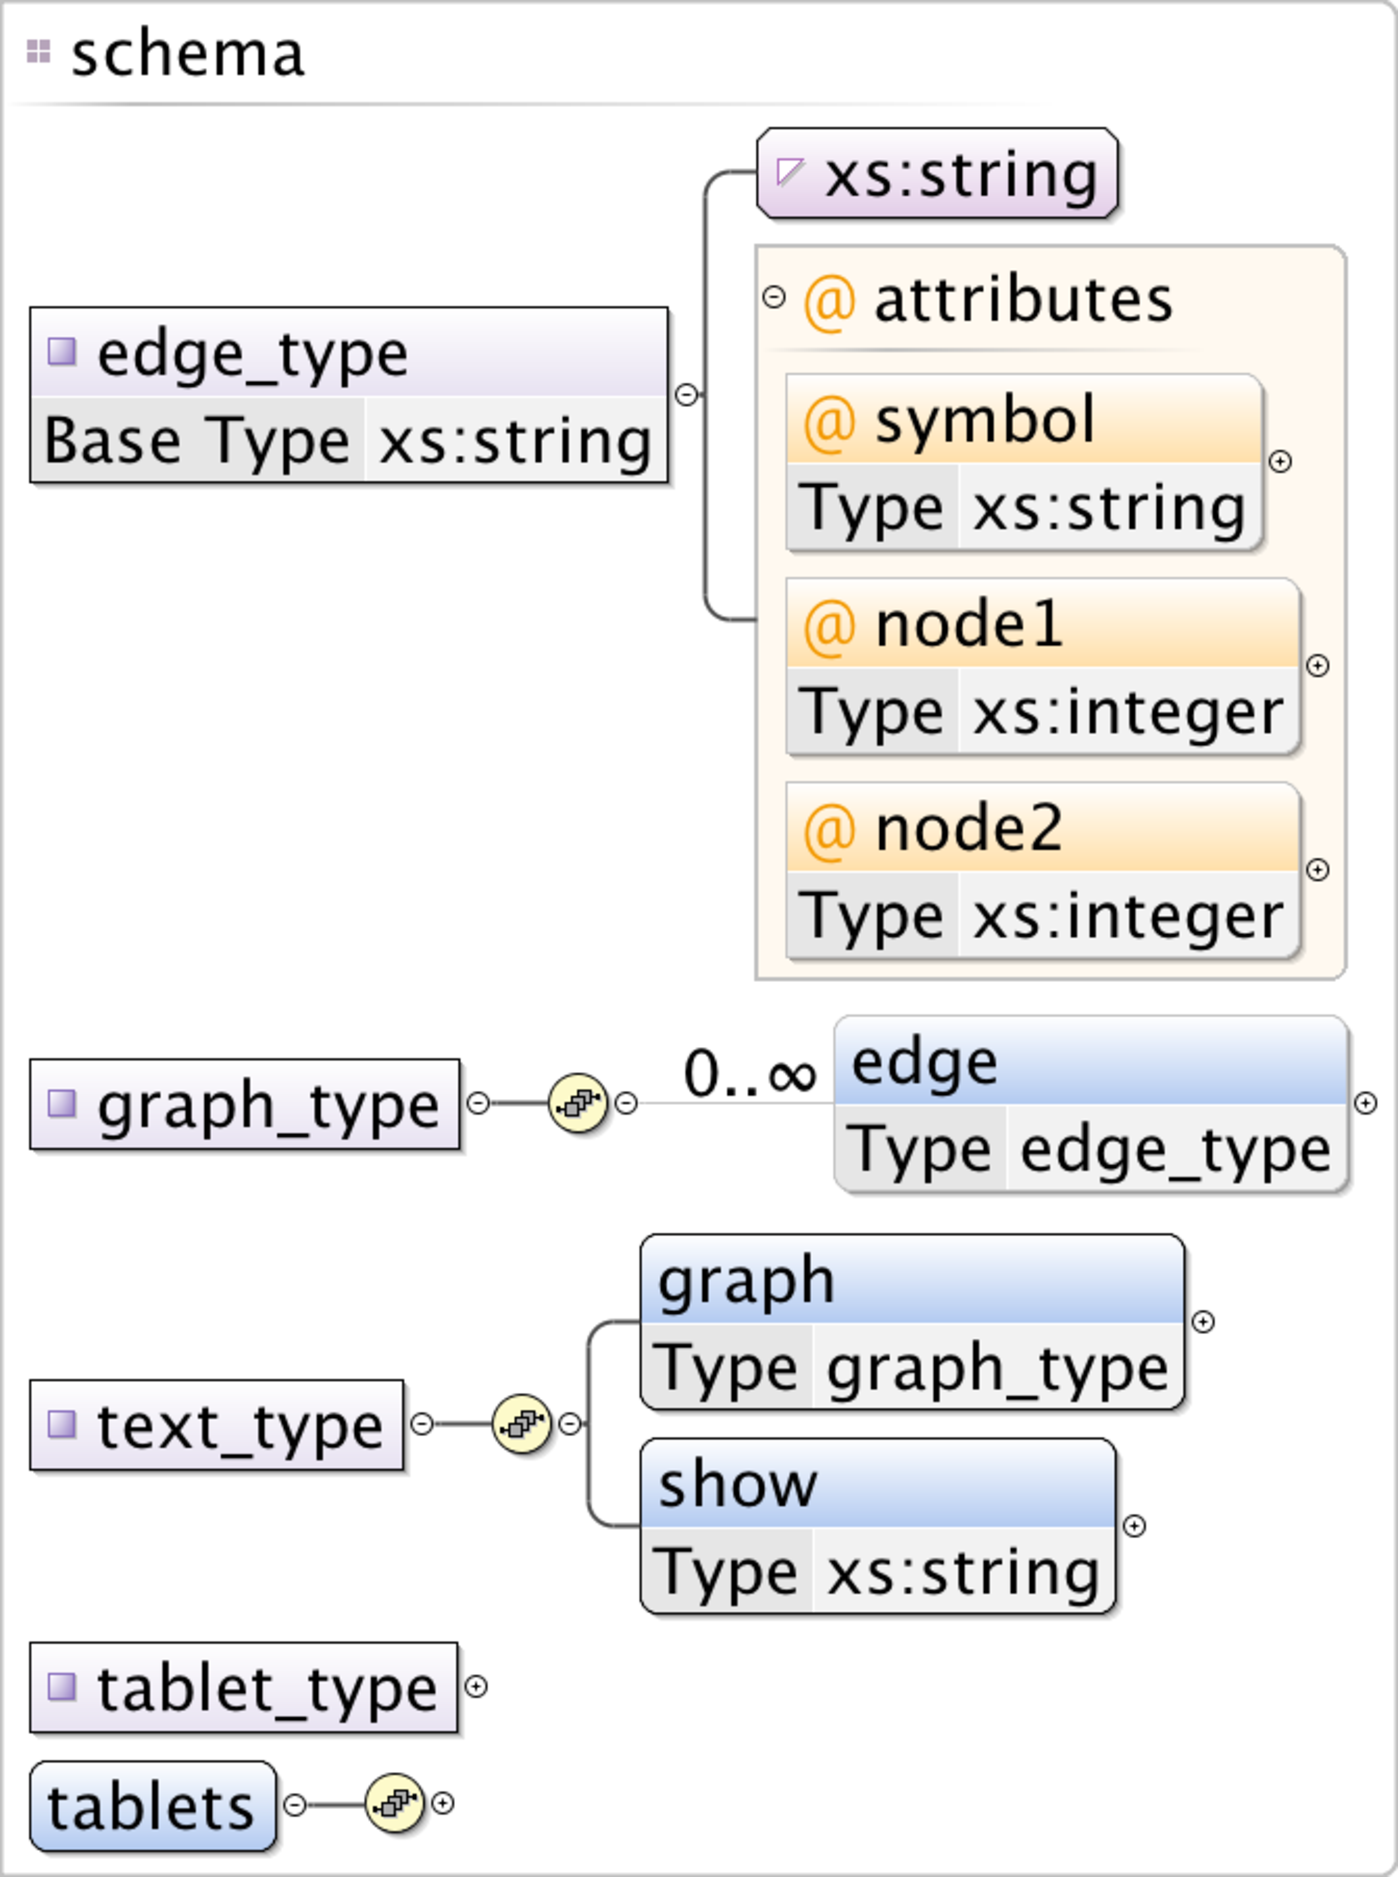
\includegraphics[width=250px]{../diagramy/schema_text.pdf}
 \caption{Schemat elementu text (kolor pomarańczowy oznacza atrybuty, a niebieski elementy)}
\end{figure}


\begin{figure}[h]
 \centering
 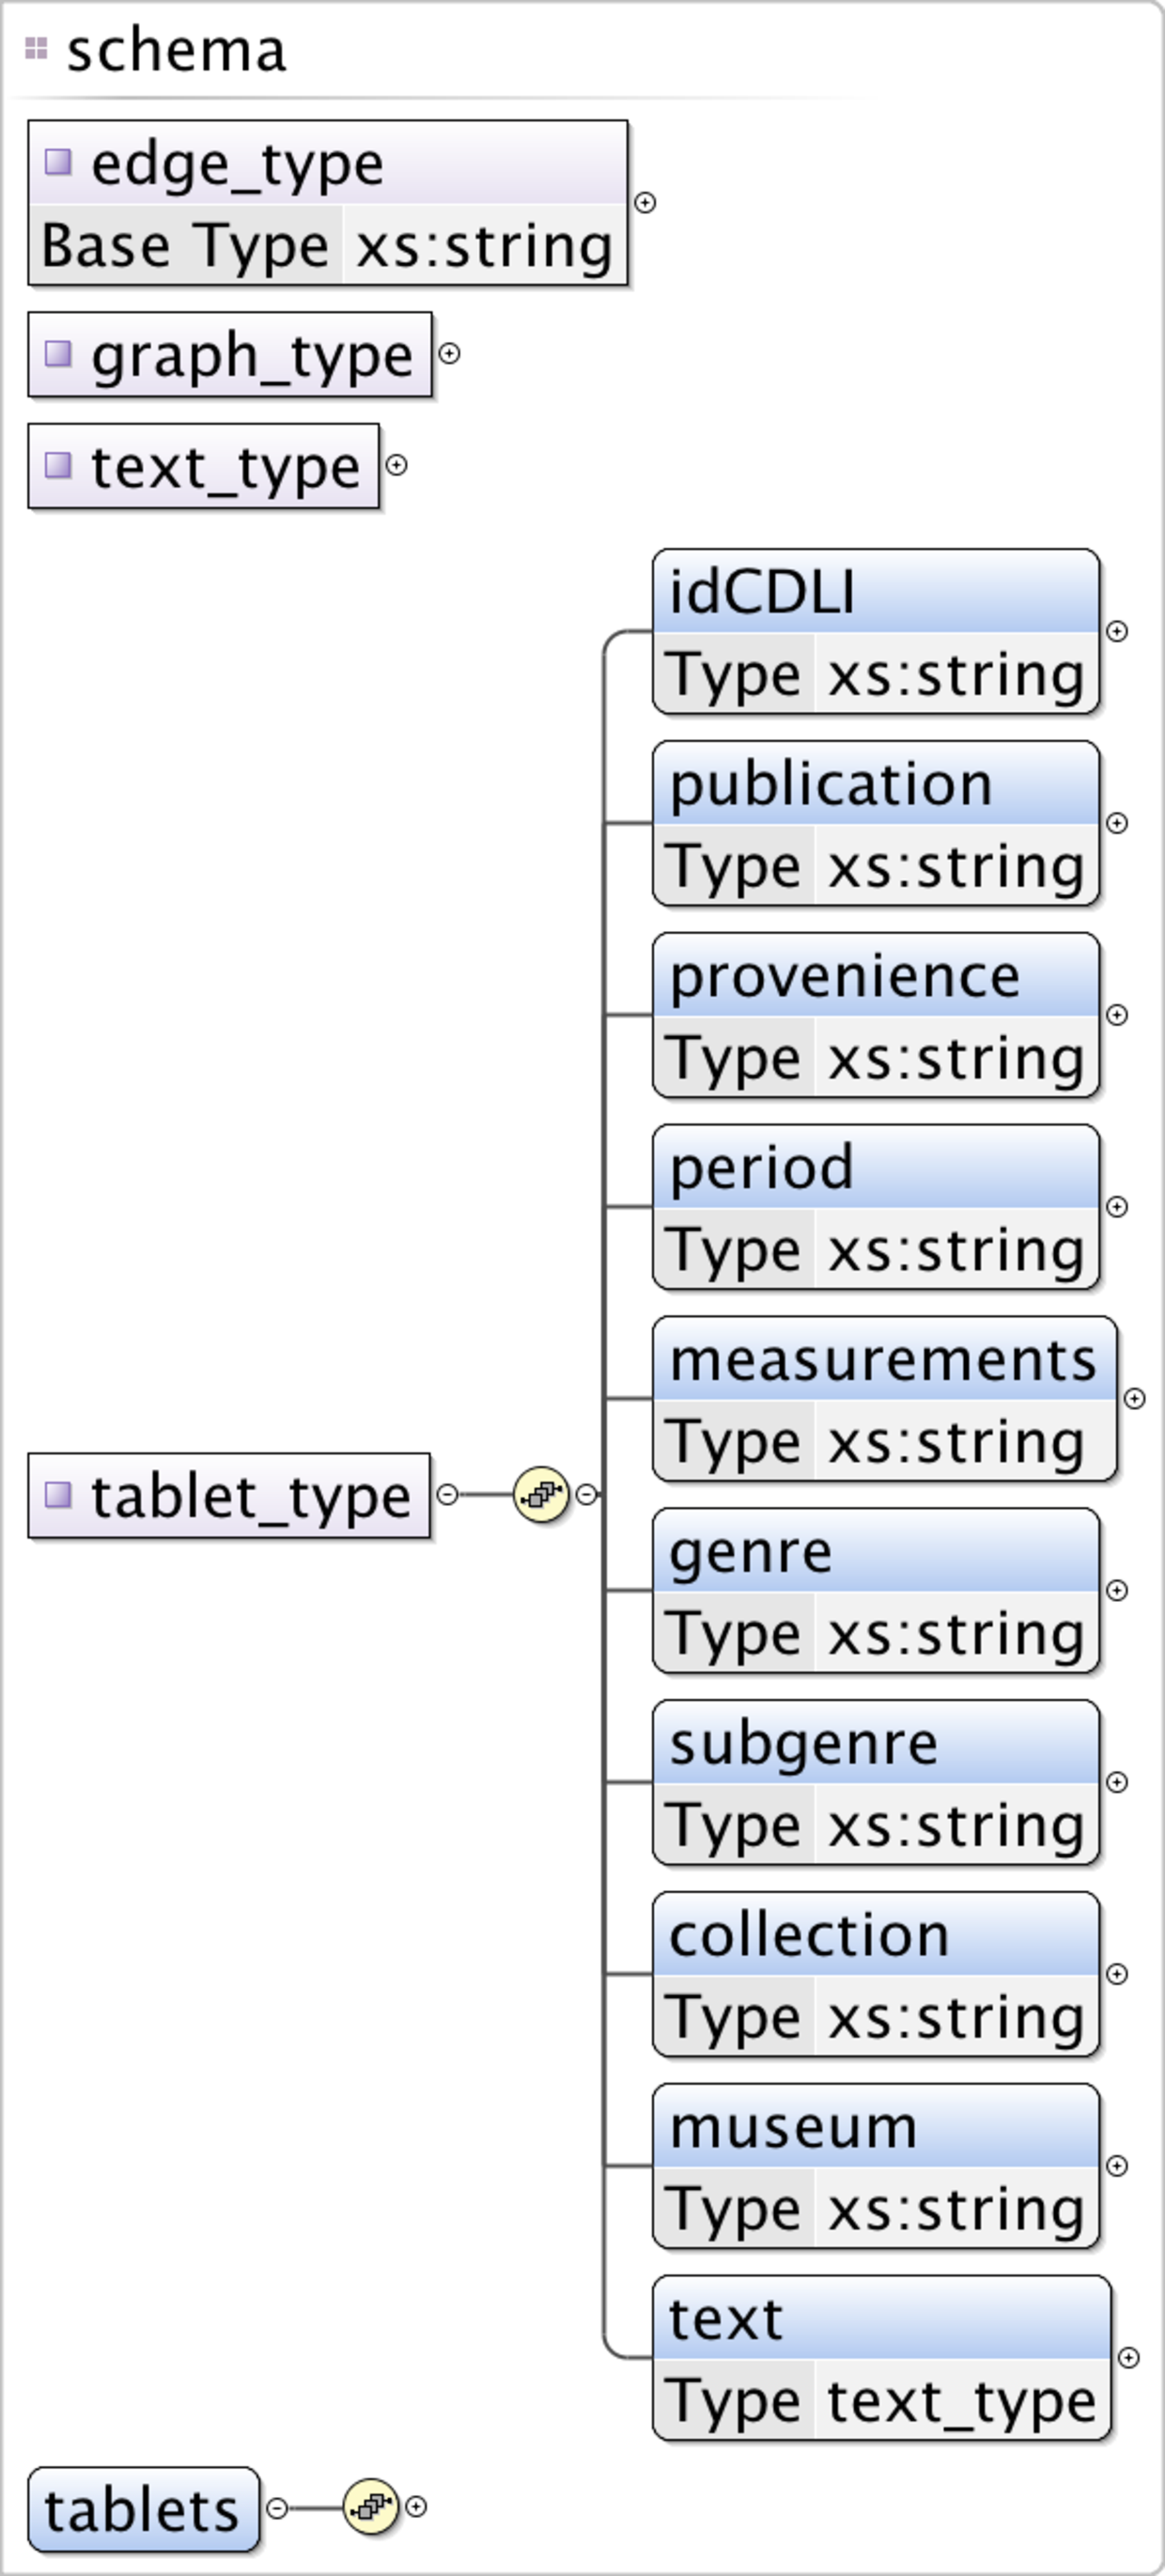
\includegraphics[width=250px]{../diagramy/schema_tablet.pdf}
 \caption{Schemat elementu tablet}
\end{figure}

\begin{figure}[h]
 \centering
 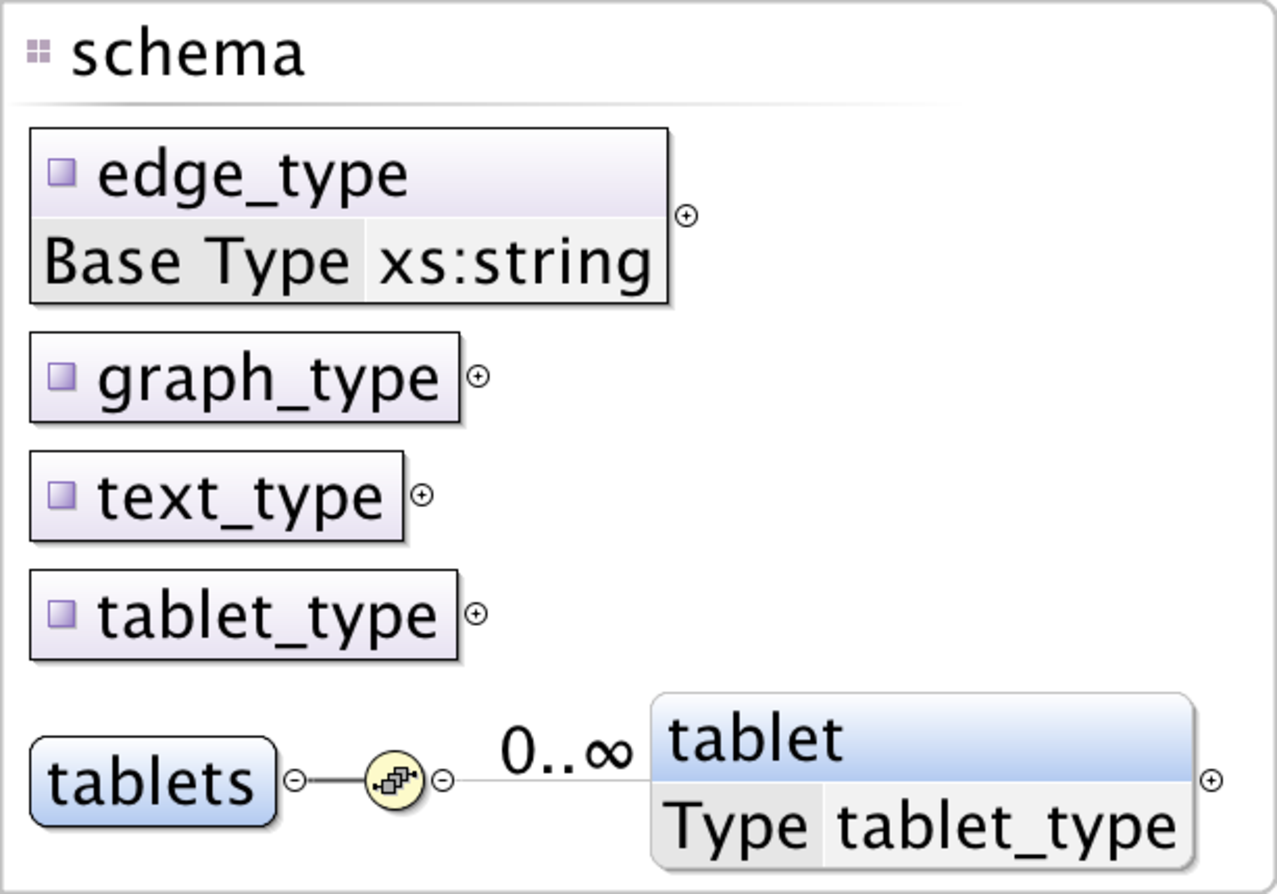
\includegraphics[width=250px]{../diagramy/schema_tablets.pdf}
 \caption{Schemat elementu tablets}
\end{figure}

Schemat dokumentu przedstawiony na obrazkach jest graficznym przedstawieniem dokumentu XML Schema (dodatek A) wygenerowanym przez program Oxygen.\\
Schemat XML jest częściowo przepisaniem diagramu encji bazy PostgreSQL. Przy tworzeniu schematu, podobnie jak w bazie relacyjnej, skorzystałyśmy z pomysłu dra Wojciecha Jaworskiego, aby przedstawić treść tabliczki w formie grafu. Każda krawędź tego grafu (odpowiadająca odczytowi) jest oddzielnym elementem, zawierającym atrybuty node1 oraz node2 - numery węzłów grafu, pomiędzy którymi się znajduje. Dodatkowo przechowujemy treść w formie napisu (element show). Metadane tabliczek przechowywane są w postaci podelementu elementu tablet. Powoduje to wielokrotne powtórzenie tych samych informacji, ale ułatwia tworzenie zapytań (?).


\subsubsection{Tłumaczenie zapytań}
Do przeszukiwania dokumentu XML wykorzystujemy język XQuery, który jest częścią rekomendacji W3C dotyczącej XML.\\
Proste zapytanie TQL tłumaczymy na pojedynczą konstrukcję FLWOR (For Let Where Order by Return).\\

\subsubsection{Stałe fragmenty}
Każde zapytanie w części For zawiera:
	\begin{verbatim}
	FOR $tablet IN .//tablet
\end{verbatim}
a w części Return:
  \begin{verbatim}RETURN <tablet>
		{$tablet/idCDLI}
		{$tablet/publication}
		{$tablet/provenience}
		{$tablet/period}
		{$tablet/measurements}
		{$tablet/genre}
		{$tablet/subgenre}
		{$tablet/collection}
		{$tablet/museum}
		{$tablet/text/show}
		<seq>...</seq>
	</tablet>
\end{verbatim}
Zawartość elementu seq zależy od ilości sekwencji, po których wyszukujemy. 

\subsubsection{Zapytania proste}

\begin{longtable}{|p{2.5in}|p{3.5in}|}
\hline
{\bf Konstrukcja} & {\bf Tłumaczenie na XQuery}\\
\hline
\endhead
provenience: wartosc & \begin{verbatim}fn:matches($tablet/provenience,'^wartosc$')\end{verbatim}
\\
\hline
publication: wartosc & \begin{verbatim}fn:matches($tablet/publication,'^wartosc$')\end{verbatim}
\\
\hline
period: wartosc & \begin{verbatim}fn:matches($tablet/period,'^wartosc$')\end{verbatim}
\\
\hline
genre: wartosc & \begin{verbatim}(fn:matches($tablet/genre,'^wartosc$')
or fn:matches($tablet/subgenre,'^wartosc$'))\end{verbatim}
\\
\hline
cdli\_id: wartosc & \begin{verbatim}fn:matches($tablet/idCDLI,'^wartosc$')\end{verbatim}
\\
\hline
\end{longtable}


\subsubsection{Treść tabliczki}
Każda sekwencja, po której wyszukujemy powoduje dodanie do zapytania następujących konstrukcji:
\begin{itemize}
\item{do części Let:}
\begin{verbatim}
let $seq <id_sekw> := (
	for $edge_end in $tablet//edge
	for $edge_start in $tablet//edge
	where (
		fn:matches($edge_start,'^<sekw[0]>$')
		and (
			some $edge1 in $tablet//edge[@node1=$edge_start/@node2]
satisfies (fn:matches($edge1,'^<sekw[1]>$')
and ... 
and fn:matches($edge_end,'^<sekw[dl_sekw-1]>$')))))
return <seq<id_sekw>> {$edge_start/@node1} {$edge_end/@node2} </seq<id_sekw>>
\end{verbatim}
\item{do części Where}
\begin{verbatim}
$seq<id_sekw>
\end{verbatim}
\item{do części Return w elemecie seq}
\begin{verbatim}
$seq<id_sekw>
\end{verbatim}
\end{itemize}




\subsubsection{Operatory}
\begin{longtable}{|p{1in}|p{3in}|}
\hline
{\bf Operator} & {\bf Tłumaczenie}\\
\hline
\endhead
/ & \begin{verbatim}(<zapytanie1> or <zapytanie2>) \end{verbatim} \\
\hline
-- & \begin{verbatim}not (<zapytanie_negowane>) \end{verbatim}\\  
\hline
+ & \begin{verbatim}(<zapytanie1> and <zapytanie2>) \end{verbatim}\\ 
\hline
* & \begin{verbatim} .*\end{verbatim}  \\ 
\hline
\end{longtable}

\subsubsection{Zapytania złożone}
Zapytanie złożone, składające się z wielu zapytań prostych tłumaczymy na sekwencję zapytań XQuery połączonych znakiem ','.

\subsubsection{Baza}
Jako bazę danych wykorzystujemy plik XML, w którym wyszukujemy za pomocą procesora XQuery Zorba. Zorba implementuje XQuery zgodnie z rekomendacją W3C.
Korzystamy z API do C++.